\chapter{Conclusions}

\section{Gateway Locations}\label{sec:gateway-locations-conclusions}

% Evaluate the chosen gateway locations and give example of the ranges, etc.
% Also add graphs of recorded gateway ranges from TTN Mapper?
This section will evaluate the chosen gateway locations as described in \cref{sec:gateway-locations} and give some examples of the ranges that can be achieved with them.
The maps used to show range data were taken from the \emph{Advanced Maps} feature of \ac{TTNM}.
Thus, as explained in \cref{subsec:cleaning-collected-data}, they may contain some inaccuracies and outliers.

\subsection{\acf{GHB} student dormitory}\label{subsec:ghb-student-dormitory-range-results}

The MikroTik gateway deployed on top of the \ac{GHB} student dormitory is the gateway with the highest range in Furtwangen.
This doesn't come as a surprise, given its exposed location on top of a hill plus the height of the building itself.

\begin{figure}[htbp]
    \centering
    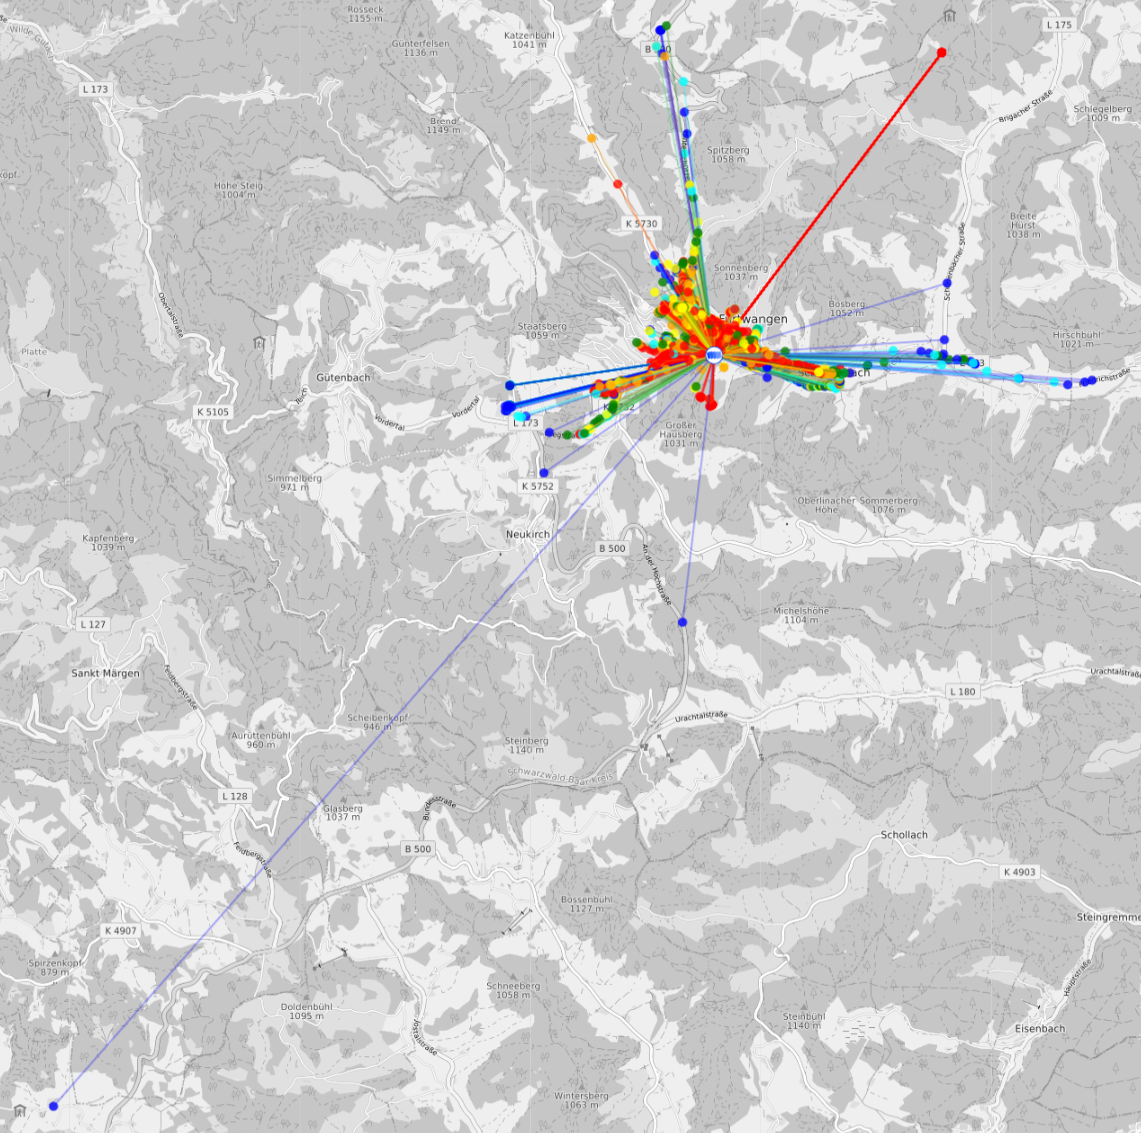
\includegraphics[width=1\textwidth]{pictures/ttn-mapper/gateway-ranges/ghb_mikrotik_gw_range.png}
    \caption{
        Map of some \ac{TTNM} data points taken from the \ac{LoRaWAN} gateway deployed on top of the \ac{GHB} student dormitory.
        The data point on the lower left is the maximum range recorded for this gateway --- \SI{14.2}{\kilo\meter}.
        However, it can be considered an outlier, as the next highest range is \SI{5.3}{\kilo\meter} away from the gateway (on the far right).
    }\label{pic:ghb_mikrotik_gw_range}
\end{figure}

The maximum range recorded for this gateway is \SI{14.2}{\kilo\meter}, which is the blue point in the lower left-hand corner of \cref{pic:ghb_mikrotik_gw_range}.
While that data point may be considered an error or outlier, a more realistic one is the blue point on the rightmost side of the image which is \SI{5.3}{\kilo\meter} away from the gateway.

\subsection{\acs{HFU} C building}

When viewed alongside the results from the \ac{GHB} gateway shown in \cref{subsec:ghb-student-dormitory-range-results}, the results from the \ac{HFU} C building gateway are exactly as one would expect.
Since the Antenna was the same MikroTik one as the one used with the \ac{GHB} gateway, the coverage behavior is similar.
The ranges as a whole are slightly lower which stems from the fact that the \ac{HFU} C building is located inside the Bregtal valley and thus has a lower elevation than the \ac{GHB} student dormitory.

\begin{figure}[htbp]
    \centering
    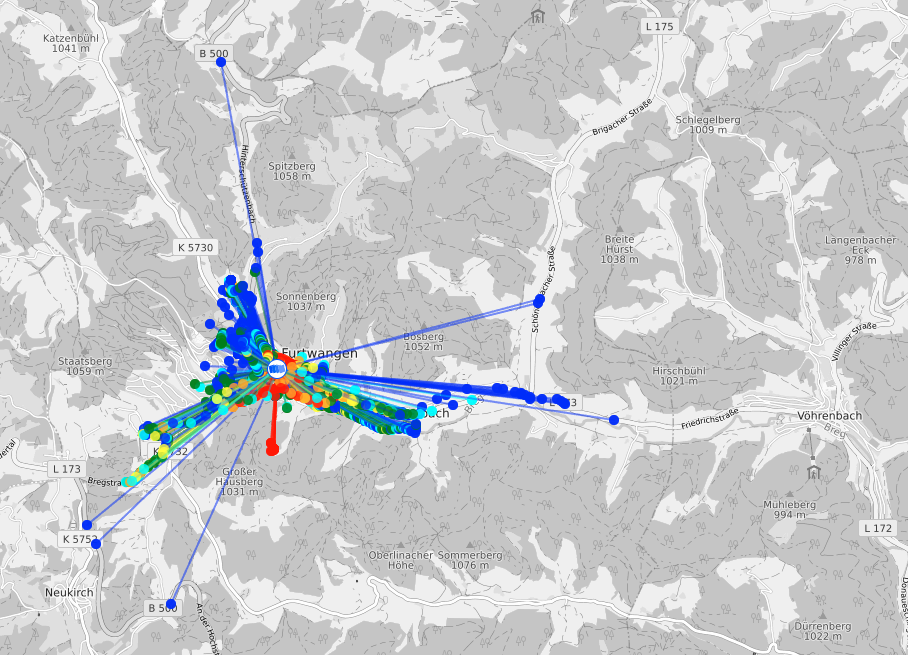
\includegraphics[width=1\textwidth]{pictures/ttn-mapper/gateway-ranges/c_building_gw_range.png}
    \caption{
        Map of some \ac{TTNM} data points taken from the \ac{LoRaWAN} gateway deployed on top of the C building.
        The slightly smaller range compared to \cref{pic:ghb_mikrotik_gw_range} is evident.
        The maximum range, however, is still \SI{4.3}{\kilo\meter} which is the rightmost blue point in the direction of Vöhrenbach.
    }\label{pic:c_building_gw_range}
\end{figure}

\Cref{pic:c_building_gw_range} shows the range of the \ac{HFU} C building gateway.
Clearly visible is the slightly smaller range compared to \cref{pic:ghb_mikrotik_gw_range}.
The maximum range recorded for this gateway is \SI{4.3}{\kilo\meter}, which is the rightmost blue point in the direction of Vöhrenbach again.

Installing the gateway on the roof of the \ac{HFU} C building was rather easy since accessing the roof is not difficult.
The cable of the antenna had to be pulled through a small conduit in the outer wall.
Afterwards, it could be connected to the \ac{LoRaWAN} gateway located inside a small crawl space.

Getting the network backhaul up and running wasn't as straightforward, though.
There were no spare Ethernet ports available in the crawl space.
However, there was a spare fiber optic cable run that was not in use at the moment.
Using two media converters, the fiber optic cable was converted to Ethernet and connected to the \ac{HFU} network one story below the roof.

\subsection{\acf{ASH}}

Installing the \ac{LoRaWAN} gateway on the roof of the \ac{ASH} building was an arduous task, but it was worth it.
The roof is difficult to access, and the gateway had to be installed on top of an antenna mast.

Getting a backhaul connection was rather easy, since a \ac{PoE} switch was available in the server room just beneath the roof.

However, the range, as shown in \cref{pic:ash_gw_range}, is very good and covers almost the entire Furtwangen area.
It is similar to the coverage of the \ac{GHB} building, since the \ac{ASH} building is also a multi-story building on a hill.

\begin{figure}[htbp]
    \centering
    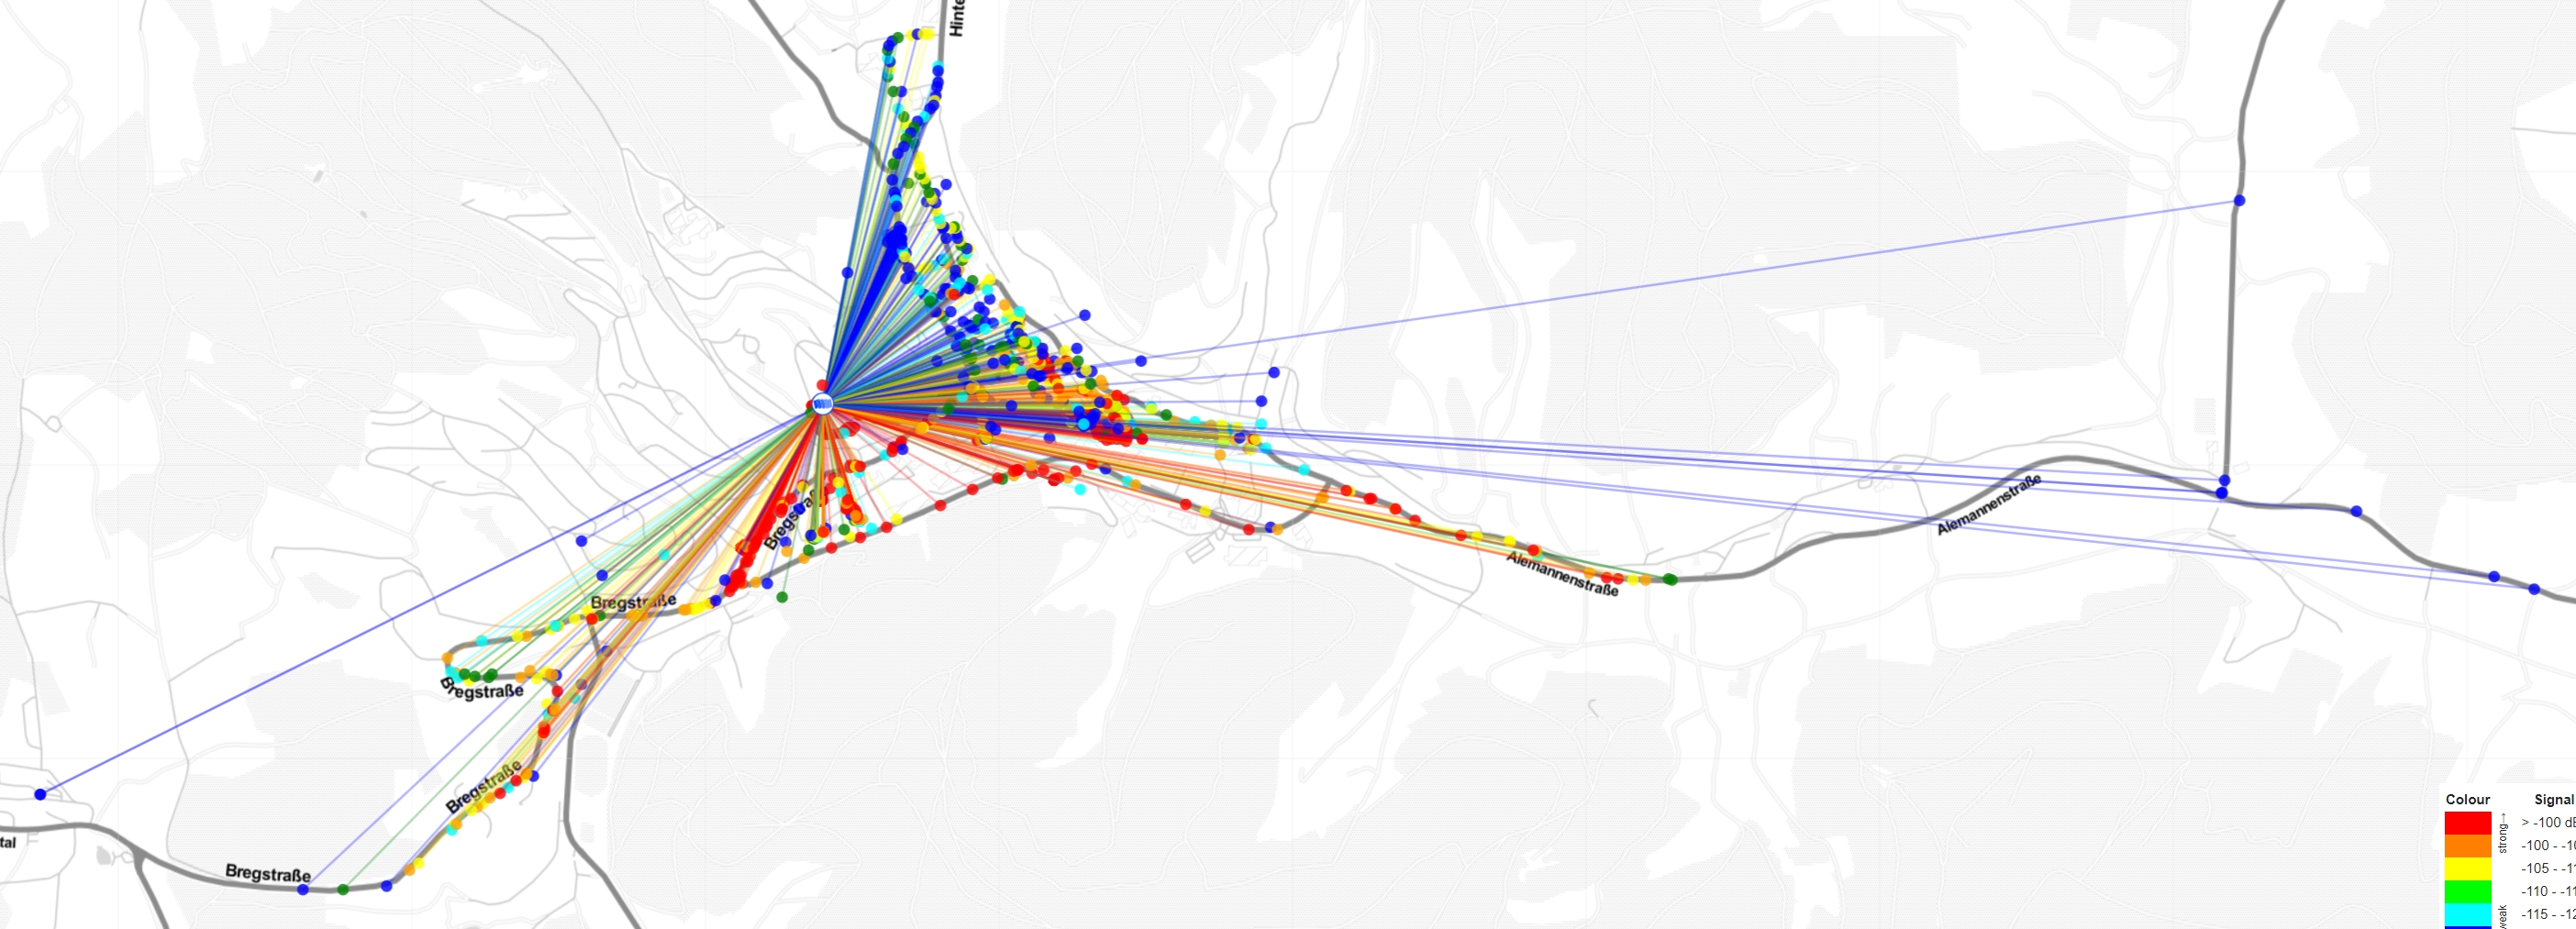
\includegraphics[width=1\textwidth]{pictures/ttn-mapper/gateway-ranges/ash_gw_range.jpg}
    \caption{
        Map of some \ac{TTNM} data points taken from the \ac{LoRaWAN} gateway deployed on the roof of the \ac{ASH} building.
        It has a good range into most parts of the Furtwangen area.
    }\label{pic:ash_gw_range}
\end{figure}

The longest range recorded from the \ac{ASH} building thus far is around \SI{4.8}{\kilo\meter} which is the blue point on the right of \cref{pic:ash_gw_range}.

\subsection{\emph{DL0FIS} amateur radio club station}

While the location of the \ac{LoRaWAN} on top of a hill between Furtwangen and Gütenbach should have made for very good coverage, the reality looks different.

\begin{figure}[htbp]
    \centering
    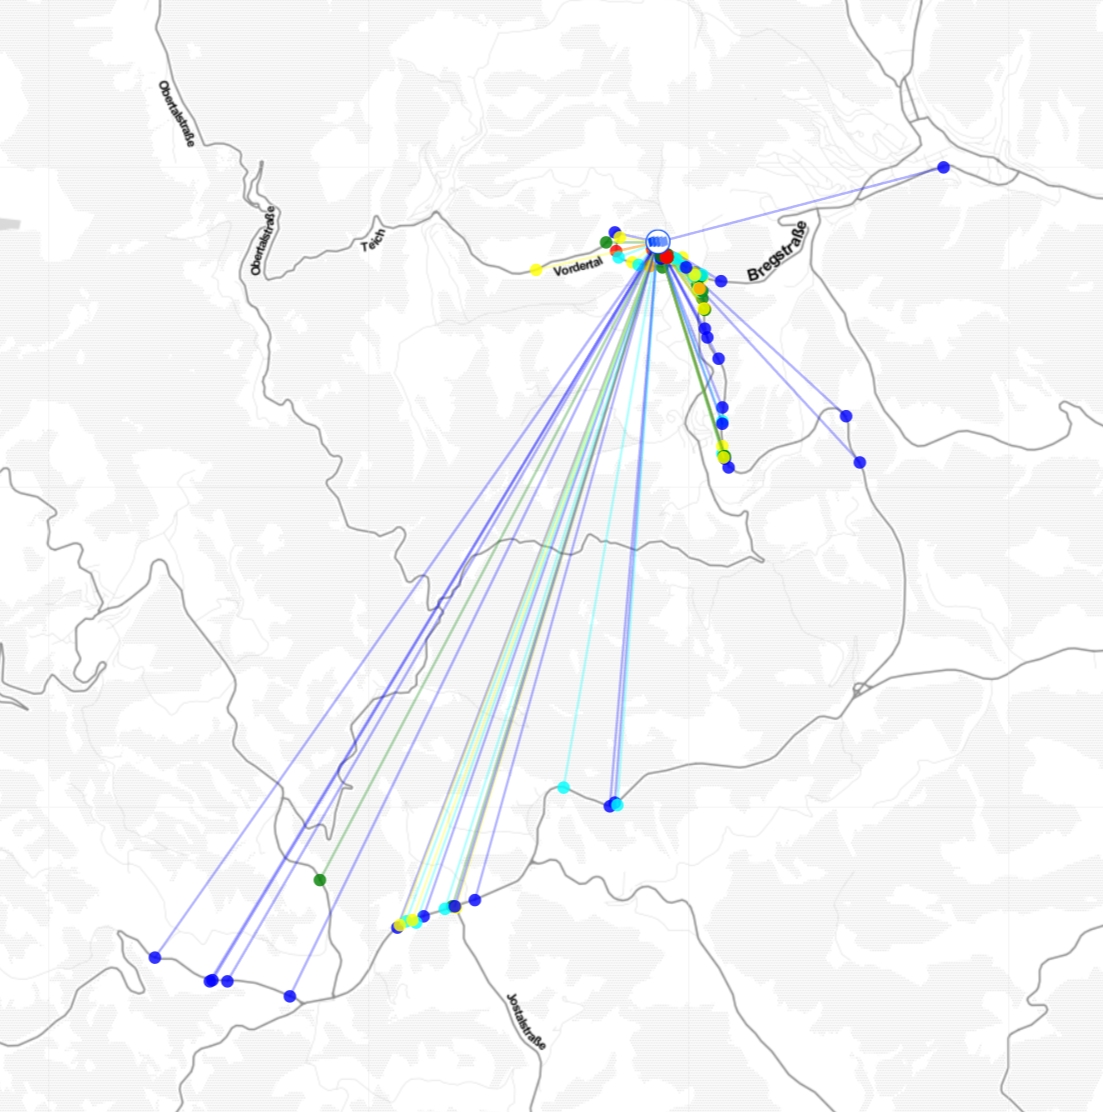
\includegraphics[width=1\textwidth]{pictures/ttn-mapper/gateway-ranges/dl0fis_gw_range.jpg}
    \caption{
        Map of some \ac{TTNM} data points taken from the \ac{LoRaWAN} gateway deployed on the roof of the \emph{DL0FIS} clubhouse.
        While the range is not consistent in every direction due to the hills and mountains in the area, the longest range of around \SI{8.8}{\kilo\meter} is still very good.
        The range to the city of Furtwangen is almost nonexistent due to the hills in the way.
    }\label{pic:dl0fis_gw_range}
\end{figure}

\Cref{pic:dl0fis_gw_range} shows the coverage of the \ac{LoRaWAN} gateway deployed on the roof of the \emph{DL0FIS} clubhouse.
The longest range measured was one data point in the south with a distance of \SI{8.8}{\kilo\meter}.
The gateway, up until now, wasn't of much use in the scope of this thesis though, since the hill between the Neueck clubhouse and the city of Furtwangen blocks most of the signal.

Getting a backhaul connection to the \ac{LoRaWAN} gateway was easy since the clubhouse is equipped with a stable internet connection.
The gateway could thus be connected using Ethernet.

\subsection{\acs{HFU} O building}\label{subsec:conclusion-hfu-o-building}

Another possible location that was not mentioned in \cref{sec:gateway-locations} was the \ac{HFU} O building.
Located in the northern part of Furtwangen, it is a multi-story building that used to be a hospital.
Since the \ac{HFU} is only a tenant there, permission was needed from the building owner to install the gateway.
Fortunately, the owner, Mr.\ Odin Jäger, was very cooperative and allowed the gateway to be installed.

Unfortunately, it was not as easy to get a network connection and power on the roof as it was in the other buildings, so no gateway has been installed there yet.

\section{Collected data in Furtwangen on \acl{TTNM}}\label{sec:collected-data-in-furtwangen-on-ttnm}

\subsection{\acl{TTNM} heatmap view after additional data collection}\label{sec:ttm_heatmap_after}

During the course of this thesis, additional data was collected using the \ac{LoRaWAN} \ac{GPS} trackers mentioned in \cref{subsec:used-lora-nodes}.
This lead to a denser data coverage of \acl{TTNM} in the Furtwangen area.

\begin{figure}[htbp]
    \centering
    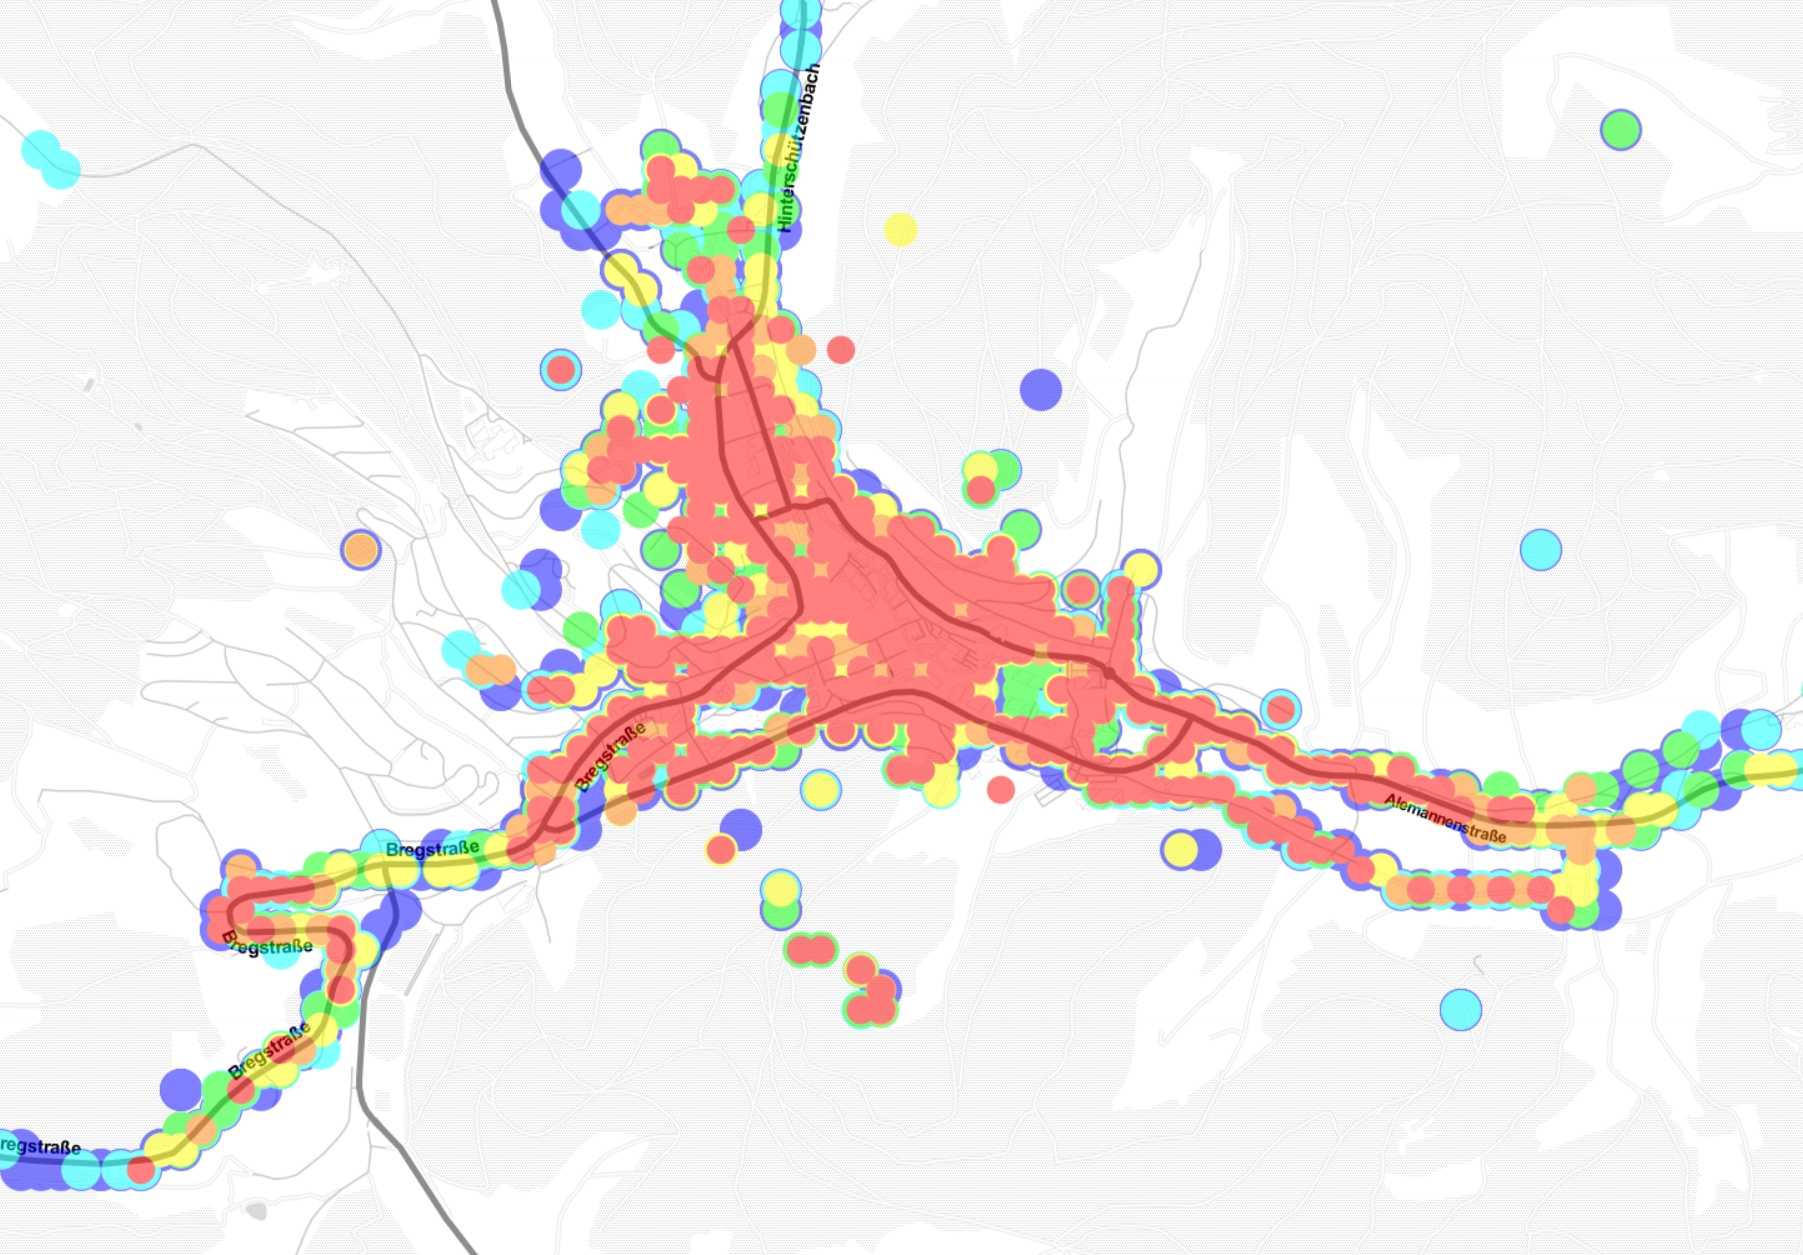
\includegraphics[width=0.7\textwidth]{pictures/ttn-mapper/ttnm_heatmap_after_data_collection.jpg}
    \caption{
        View of the \ac{TTNM} heatmap view after data collection during this thesis, from the 21st of June 2023.
        Compared to \cref{pic:ttnm-before-data-collection}, the coverage is better.
        This is due to the fact that several \ac{LoRaWAN} gateways were deployed during this thesis as well as the additional data collection performed with \ac{LoRaWAN} \ac{GPS} trackers.
    }\label{pic:ttnm-heatmap-after-data-collection}
\end{figure}

\Cref{pic:ttnm-heatmap-after-data-collection} shows a view of the \ac{TTNM} heatmap after the additional data collection that was done during this thesis.
The much redder color of the map is visible, meaning that the signal strength in these areas is stronger than before.

While there are still some blank spots, these are mostly due to the fact that these areas were not visited by \ac{GPS} trackers during the data collection in this thesis.

\section{Comparison of Geolocation Methods}

This section will compare the different geolocation methods that were used in this thesis.

\subsection{\acf{RSSI}}

% TODO: mention the problems with RSSI-based geolocation (different antennas per gateway, different antennas per node, different environments, etc.)

\subsubsection{Accuracy of \acs{RSSI}-based geolocation with linear regression per gateway}\label{subsubsec:conclusion-rssi-linear-regression}

\subsection{\acf{ToA}}\label{subsec:conclusion-toa-tdoa}

\Cref{subsec:toa-based-multilateration-implementation} mentioned the fact that using timestamps from a \ac{LoRaWAN} gateway to determine the range to the end device is too inaccurate to be used for \ac{ToA}-based geolocation.

In addition to the fact that timestamps arrive at \ac{TTN} with unrealistic offsets due to missing time synchronization, another factor has to be considered.
The device timestamps arrive at \ac{TTN} in a format such as \texttt{2023-06-23T15:11:11.678179Z}.
The six decimal places after the seconds mean that the timestamp is accurate to \SI{1}{\micro\second}.
\Cref{eq:toa-accuracy-ttn-microseconds} shows that when using microseconds to calculate the distance to a \ac{LoRaWAN} gateway based on the speed of light, a maximum accuracy of \SI{300}{\meter} can be achieved.

\begin{equation}\label{eq:toa-accuracy-ttn-microseconds}
    \text{accuracy}_{\si{\micro\second}} = \frac{299792458 \frac{\si{\meter}}{\si{\second}}}{10^6} \approx 300 \si{\meter}
\end{equation}

\Cref{eq:toa-accuracy-ttn-nanoseconds} shows that using nanoseconds, a much better accuracy of \SI{0.3}{\meter} could be achieved.

\begin{equation}\label{eq:toa-accuracy-ttn-nanoseconds}
    \text{accuracy}_{\si{\nano\second}} = \frac{299792458 \frac{\si{\meter}}{\si{\second}}}{10^9} \approx 0.3 \si{\meter}
\end{equation}

Solving this problem on the scope of the entire \ac{TTN} \ac{LoRaWAN} network is not feasible as it would entail synchronizing the clocks of all gateways in the network with \ac{GPS} receivers.
However, if one were to deploy a \ac{LoRaWAN} network in a smaller area where control over every reachable gateway is realistic, this would be a possible solution.
If every gateway in the network is time-synchronized, \ac{ToA} could be used for geolocation.

% TOOD sources

\subsection{Fingerprinting}

% TODO: describe how this worked and how it could be improved (worked pretty okay but has only limited accuracy)

% TODO: mention the potential of using machine learning to improve the fingerprinting method

\section{Comparison of findings with existing work}

% TODO mention the existing work in conjunction with my own findings as far as localization is concerned

\section{Problems}

\subsection{Falsely entered gateway locations}

% Mention problems with falsely entered gateway locations and how they could be fixed

\section{Outlook}

% TODO: What else can be done? What are the next steps?

\subsection{Improving the \acf{TTNL} software}

% TODO: show what else could be done - automatically recognize if gateways moved too far away like in TTN Mapper etc.

\subsubsection{Automatically detecting moved gateways}

% TODO write about this

\subsubsection{Remove dependency on \acl{TTNM}}

Since this thesis is largely based on \ac{TTNM}, it would be beneficial to remove the dependency on it.
Should \ac{TTNM} ever be discontinued, the \ac{TTNL} software would no longer be able to function in its current state.
A taste of such a situation was already experienced during the development of this thesis, when the \ac{TTNM} \ac{API} was down for several hours one day during the development phase.

To remove the dependency on \ac{TTNM}, the \ac{TTNL} software could be extended to include its own \ac{REST} endpoints, providing the same ability to receive data directly from \ac{TTN} as \ac{TTNM}.
This would enable the \ac{TTNL} software to function without \ac{TTNM} and would also allow for more flexibility in data collection in the future.

\subsubsection{Better sharing of type definitions between Frontend and Backend}\label{subsubsec:outlook-sharing-type-definitions}

% TODO: two repos, some duplicate type files, could be improved

\subsubsection{Choice of technologies}

% TODO: could have used SvelteKit oder Nuxt.js to have the entire project in one repo
% enables better type sharing, etc.

\subsubsection{Recognizing moving gateways}

Currently, the backend of the \ac{TTNL} software cannot recognize if a gateway has moved its position since the last time it was captured.
This can lead to problems when the gateway is moved to a different location, as the software will still use the old location for the gateway and assumes that its previous data
points were captured at the same location.
\ac{TTNL} could be improved by adding a feature that recognizes if a gateway has moved and then deletes all data points that were captured at the old location of the gateway.

\subsection{Projects made possible due to better \acs{LoRaWAN} coverage in Furtwangen}

As there are now several new \ac{LoRaWAN} gateways in Furtwangen, there are several projects that can be done in the future that would not have been possible before without installing such gateways by oneself.

This section will list some of these projects and describe how they could be implemented.

\subsubsection{Measuring the water level of the Breg river}

One of the \ac{LoRaWAN} nodes ordered as part of this thesis is a \emph{Milesight EM310-UDL}, an ultrasonic distance/level sensor.
As the \ac{LoRaWAN} network coverage of Furtwangen is now adequate, it would be possible to use this sensor to measure the water level of the Breg river flowing through the vicinity of the \ac{HFU}.
This would allow for a more accurate prediction of the water level of the Breg river, which might in turn allow for a more accurate prediction of the water level of the Danube river.
Installing this \ac{LoRaWAN} node as well as connecting it to \ac{TTN} and adding an \acf{AS} to it to allow monitoring of the water level of the Breg river would be a good future project for students of the \ac{HFU}, enabled by the gateways placed during this thesis.

\subsubsection{Measuring soil moisture and environmental conditions in the Furtwangen city park}

This same semester, Samuel Kasper, a student of the \ac{DM} faculty of the \ac{HFU} wrote his bachelor thesis about measuring the humidity as well as the temperature of the soil to monitor plants and crop growth.
The installation of \ac{LoRaWAN} gateways in the city of Furtwangen helped him in this regard, as he did not have to install his own gateways and instead could use the now existing infrastructure in the city.

\subsubsection{Monitoring of Gateways}

Another possible project would be an application that monitors the gateways and checks if they are still online.
Such a project could be realized with software like \emph{Node-RED}.

\subsection{Further research}

\subsubsection{Improving timestamp accuracy for \acf{ToA} geolocation method}

As mentioned in \cref{subsec:conclusion-toa-tdoa}, the accuracy of the \ac{ToA} method could be greatly improved if nanosecond level timestamps were available.
Unfortunately, \ac{TTN} does not provide nanosecond level timestamps for the packets received by the \ac{LoRaWAN} gateways.
To solve this problem, a \ac{LNS} would need to be set up that has the ability to do that.

In addition, \ac{LoRaWAN} gateways would need to be time synchronized to achieve the best possible accuracy.
The latter problem could be solved by using \ac{GPS} receivers to synchronize the gateways.
While some gateways have \ac{GPS} built-in receivers, most do not.
For example, the \emph{Dragino DLOS8N} that was used twice during this thesis has a \ac{GPS} built-in receiver~\cite{dragino_technology_co_ltd_dlos8n_2023}, but none of the others do.

In any case, using the \ac{ToA} method would require more specific hardware than what most of the \ac{TTN} community network currently uses.
This makes it unsuitable for widespread use on that particular network.

\subsubsection{Using \acf{ML} to improve the fingerprinting method}


There are several \ac{ML} methods that could be used to improve the fingerprinting method.
For example, \ac{kNN} could be used to determine the location of a node based on the \ac{RSSI} values of the surrounding gateways~\cite{anagnostopoulos_reproducible_2019}.

\subsubsection{Also use \ac{SF} and \ac{SNR} values for fingerprinting}

As mentioned in \cref{sec:sf-snr-correlation}, the \ac{SF} used by the end device has an influence on the \ac{SNR} values at which a signal can still be detected.
This means that the \ac{SF} and \ac{SNR} values used by the end device could also be used to more accurately determine the location of the end device.
Since the \ac{TTN} data frames include this information, it could be used to improve the fingerprinting method.

A disadvantage of this approach would be that it would require more data to be collected, since the number of possible variables per captured gateway would increase from 1 (\ac{RSSI}) to 3 (\ac{RSSI}, \ac{SF}, \ac{SNR}).

\subsubsection{Gateway on the roof of the \acs{HFU} O building}

As was mentioned in \cref{subsec:conclusion-hfu-o-building}, the roof of the O building would make another good location for a \ac{LoRaWAN} gateway.
The permission by the building's owner was granted.
The problem that would need to be solved is getting a network connection as well as power to the roof of the building.

Another option that would only require getting power to the roof is to use a \ac{LoRaWAN} gateway that has a \ac{LTE} backhaul connection.
However, getting a \ac{PoE} connection to the roof of the building would still be preferable due to its stability.

\subsubsection{Self-hosting of \acs{TTS} or \emph{ChirpStack}}

Another interesting project would be to self-host an instance of a \ac{LNS} like \ac{TTS} or \emph{ChirpStack} on \ac{HFU} infrastructure.
This would give students the opportunity to learn more about the inner workings of a \ac{LNS} and would also give the \ac{HFU} the ability to exert more control over the data collected by the \ac{LNS}.
Both of them are \ac{OSS} and can be self-hosted using Docker or Docker Compose.

\subsubsection{Privacy concerns}

% TODO: write about privacy concerns with geolocation and tracking of people

% Notes:
% Geräte können verfolgt werden (tracking)
% - ggf. "welche Personen haben welche Geräte?"
% - Geräte halten ewig und können aufgrund ihrer Größe leicht versteckt werden

% Actually: Maybe mention how the gateway on top of the E. Wehrle Building could be located with just a bit of data collection?